%\documentclass[dvipdfmx,xcolor={svgnames},17pt]{beamer}
\documentclass[dvipdfmx,xcolor={svgnames}]{beamer}

\usepackage{pxrubrica}
\usepackage{color}
\usepackage{tikz}
\usepackage{pgfplots}
\usepackage{amsmath}
\usepackage{amsfonts}
\usepackage{ifthen}
\usepackage{minted}

\usetheme{Copenhagen}
\usecolortheme{whale}

\setbeamertemplate{caption}[numbered]
\setbeamertemplate{footline}[frame number]

\setbeamerfont{title}{size = \Huge}
\setbeamerfont{subtitle}{size = \huge}
\setbeamerfont{date}{size = \huge}
\setbeamerfont{author}{size = \huge}
\setbeamerfont{frametitle}{size = \huge}
\setbeamerfont{normal text}{size = \Large}
\setbeamerfont{block body}{size = \Large}
\setbeamerfont{item}{size = \Large}
\setbeamerfont{enumerate}{size = \Large}


\renewcommand{\figurename}{図}
\renewcommand{\tablename}{表}

\graphicspath{{./img/}}

\pgfplotsset{
  integral axis/.style={
        axis lines=middle,
        enlarge y limits=upper,
        axis equal image, width=12cm,
        xlabel=$x$, ylabel=$y$,
        ytick=\empty,
        xticklabel style={font=\small, text height=1.5ex, anchor=north},
        samples=100
        },
        integral/.style={
            domain=2:10,
            samples=9
            },
            integral fill/.style={
            integral,
            draw=none, fill=#1,
            on layer=axis background
            },
            integral fill/.default=cyan!10,
            integral line/.style={
            integral,
            very thick,
            draw=#1
            },
            integral line/.default=black
}

\def\vector#1{\mbox{\boldmath $#1$}}

\renewcommand{\kanjifamilydefault}{\gtdefault} % 日本語書体をゴシック体に
\renewcommand{\familydefault}{\sfdefault} % 欧文書体をHelveticaに

\newminted[GAS]{javascript}{linenos}

\title{SAMIT18.05}
\subtitle{GASによる初めてのボット作成}
\author{17043052 藤原 渓亮}
\date{2018年5月26日}

\begin{document}
  \maketitle
  \begin{frame}{今日やること}
    \begin{center}
      \Huge ボット作ります
    \end{center}
  \end{frame}
  \begin{frame}{今日やること}
    \huge こんな感じです.
    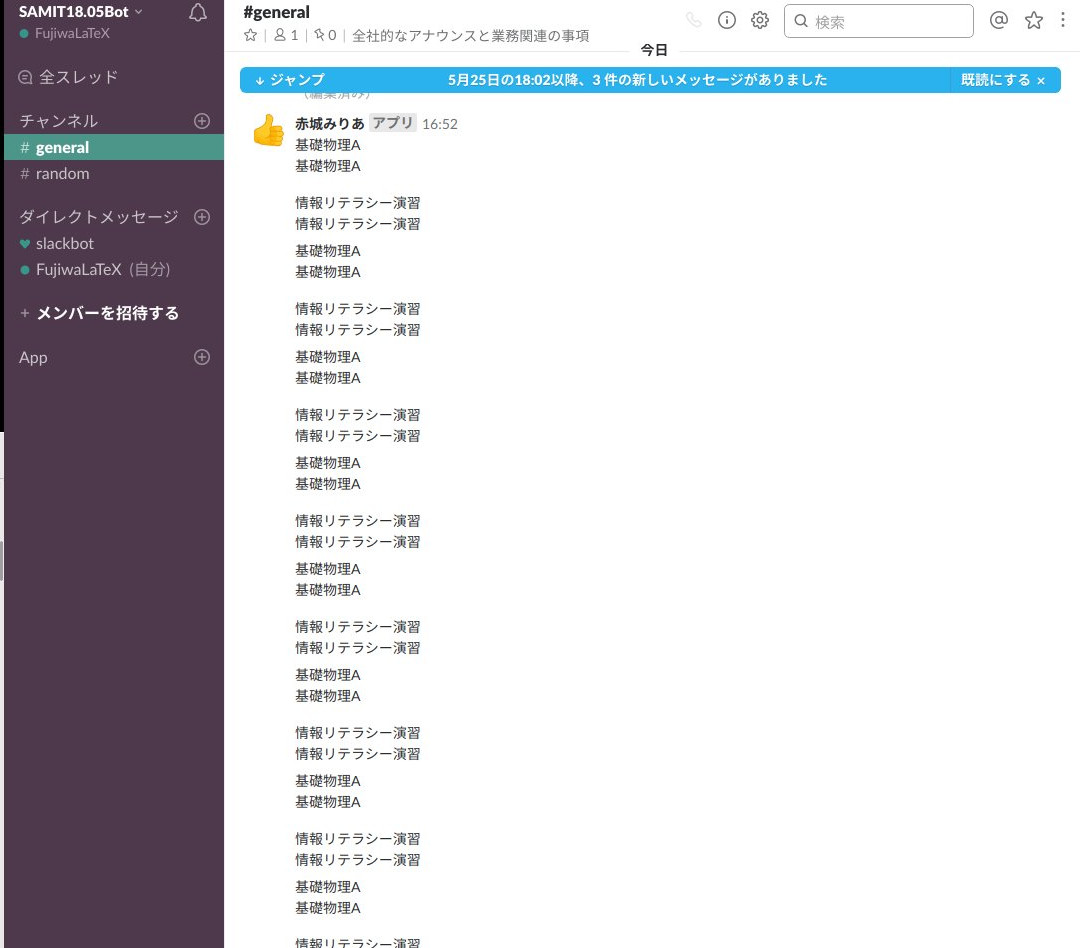
\includegraphics[width=\hsize]{sc01.jpg}
  \end{frame}
  \begin{frame}{今日やること}
    \huge Slack(チャットツール)に定期的に時間割を
    通知してくれるボットを作ります.
  \end{frame}
  \section{Slack側の準備}
  \begin{frame}{Slackの用意}
    \begin{block}{Slackとは}
      Slack Technologies社が開発した
      ビジネス向けチャットツール
    \end{block}
    \begin{figure}\centering
      
\includegraphics[width=\hsize]{slack_cmyk.pdf}
    \end{figure}
  \end{frame}
  \begin{frame}
    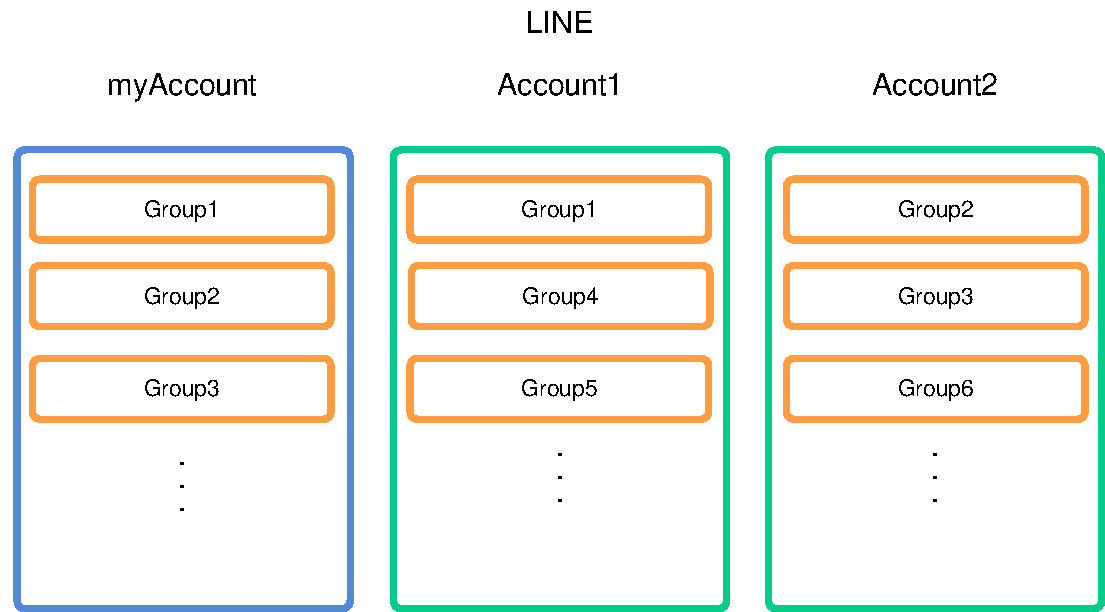
\includegraphics[width=\hsize]{LINE_image_figure.pdf}
    \pause\huge 一つのアカウントが \\ 複数のグループに所属
  \end{frame}
  \begin{frame}
    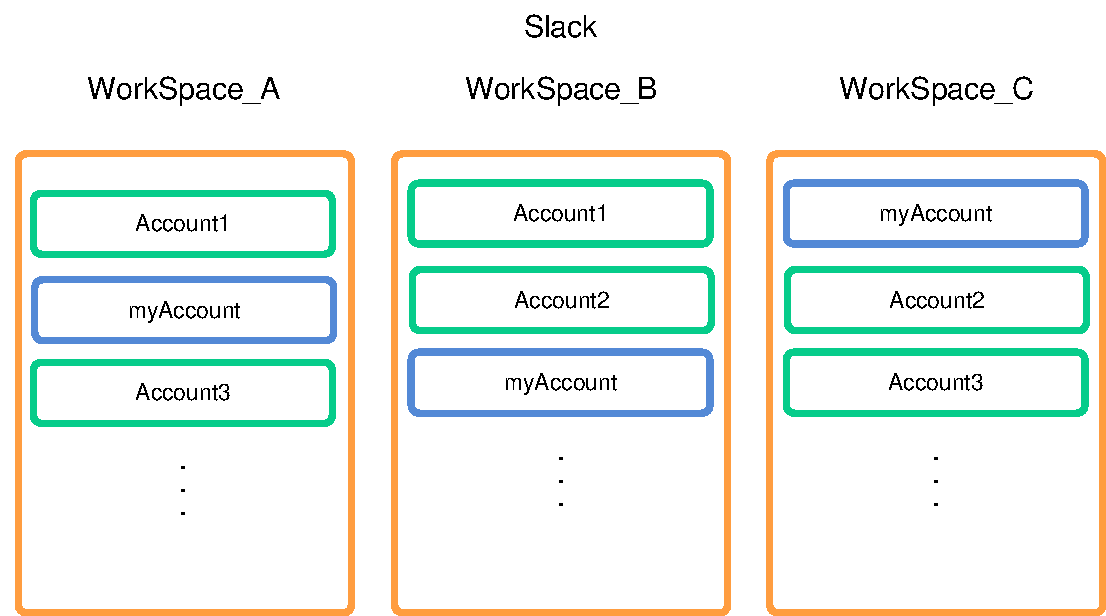
\includegraphics[width=\hsize]{Slack_image_figure.pdf}
    \pause\huge グループ毎にアカウントを持つ
  \end{frame}
  \begin{frame}{ワークスペース作成}
    \begin{enumerate}\Large\setlength{\itemsep}{15pt}
      \item \url{https://slack.com/intl/ja-jp}にアクセス
      \item 右上の「ワークスペース」をクリック
      \item 最下部にある「ワークスペースの作成」 \\ をクリック
    \end{enumerate}
  \end{frame}
  \begin{frame}{アプリ追加}
    \begin{enumerate}\Large\setlength{\itemsep}{15pt}
      \item チャット画面から「+アプリ追加」をクリック
      \item ``incomming web hook''で検索
      \item 「設定を追加」をクリック
    \end{enumerate}
    \begin{block}{着信Webフック}
      外部からSlackにメッセージを送れるアプリ
    \end{block}
    \onslide<2>{投稿するチャンネルを決めたら「インテグレーションの追加」}
  \end{frame}
  \begin{frame}[fragile]{Slackにメッセージを送ってみる}
    \begin{exampleblock}{コマンドラインからメッセージを送信}
      \begin{GAS*}{fontsize=\Large}
curl -X POST --data-urlencode
"payload={\"text\": \"Hello Slack\"}"
<your Webhook URL>
\end{GAS*}
    \end{exampleblock}
    \onslide<2>{Windowsはcurlコマンドありません.}
  \end{frame}
  \section{GAS側の準備}
  \begin{frame}{Googleスプレッドシートをオリジナル時間割にする}
    \begin{block}{スプレッドシートをコピー}
      \begin{enumerate}\setlength{\itemsep}{15pt}
        \item \url{https://goo.gl/ec1Gmk}からスプレッドシートにアクセス
        \item 「ファイル」 $\rightarrow$ 「コピーを作成」
        \item 自分のディレクトリに保存
        \item コピー先で時間割カスタマイズ
      \end{enumerate}
    \end{block}
    {\huge エクセルと使い方はほぼ一緒}
    \end{frame}
  \begin{frame}{GASについて}
    \begin{block}{GASとは}
      Google Apps Scriptの略で,Googleのサービスを操作できる環境.
      言語はJavaScript
    \end{block}
    \begin{block}{GASから利用できるサービス}
      Googleスプレッドシート,Googleドキュメント,Googleスライドの
      データ操作や取得,Gmailへ通知を送信などが可能
    \end{block}
  \end{frame}
  \begin{frame}{スプレッドシートにGASを導入}
    \begin{enumerate}  \setlength{\itemsep}{20pt}\LARGE
      \item コピーしたスプレッドシートを開く
      \item 「ツール」 $\rightarrow$ 「スクリプトエディタ」
    \end{enumerate}
  \end{frame}

  \begin{frame}[fragile]{GASを書く}
    \begin{exampleblock}{Hello World!!}
      \begin{GAS}
function helloWorld(){
  Logger.log("Hello World!!");
}
      \end{GAS}
    \end{exampleblock}
    \begin{block}{スクリプト実行}
      \begin{enumerate}
        \item 「実行」$\rightarrow$「関数を実行」$\rightarrow$ ``helloworld''
        \item ctrl + Enterでログ確認
      \end{enumerate}
    \end{block}
  \end{frame}

  \begin{frame}[fragile]{GASを書く}
    \begin{exampleblock}{スプレッドシートからデータ取得}
      \begin{GAS*}{fontsize=\scriptsize}
function helloWorld(){
  Logger.log("Hello World!!");
}
function getSheetInfos(){
  const values = SpreadsheetApp.getActiveSheet().getRange("A1").getValues();
  return values;
}
      \end{GAS*}
    \end{exampleblock}
    \LARGE A1セルから値を取得して,ログに出力(ctrl+Enterで見れる)
  \end{frame}
  \begin{frame}[fragile]{GASからSlackへメッセージを送る}
    \begin{exampleblock}{GASからPOSTリクエストを送る}
      \begin{GAS*}{fontsize=\small}
function postSlack(text){
  const url = "<your Webhook URL>";
  const options = {
    "method" : "POST",
    "headers": {"Content-type": "application/json"},
    "payload" : JSON.stringify({"text": text})
  };
  UrlFetchApp.fetch(url, options);
}
      \end{GAS*}
    \end{exampleblock}
    \begin{onlyenv}<2>
      \begin{exampleblock}{送るメッセージを受け取る関数}
        \begin{GAS}
function test(){
  postSlack("これはテストです");
}
        \end{GAS}
      \end{exampleblock}
    \end{onlyenv}
    \begin{onlyenv}<3>
      \begin{block}{UrlFetchApp.fetch}
        urlで指定した場所にoptionsで指定した条件で
        データを送る
      \end{block}
    \end{onlyenv}
    \begin{onlyenv}<4>
      \begin{block}{url}
        データを送る先
      \end{block}
    \end{onlyenv}
    \begin{onlyenv}<5>
      \begin{block}{options}
        \begin{description}\normalsize
          \item[method] HTTPリクエストの種類
          \item[headers] 送るデータの形式
          \item[payload] 送るデータの内容
        \end{description}
      \end{block}
    \end{onlyenv}
    \begin{onlyenv}<6>
      \begin{block}{JSON}
        データ記述言語の一種(データ構造を表す)
      \end{block}
    \end{onlyenv}
  \end{frame}

  \begin{frame}[fragile]{月曜日の時間割をSlackに通知してみる}
    月曜日の時間割 $\rightarrow$ B2からB11
    \begin{exampleblock}{月曜日の時間割を返す関数}
      \begin{GAS}
function notifyMondaySchdule(){
  const classes = getSheetInfos("B2:B11");
  const todayScheduleStr = listToStr(classes);
  postSlack(todayScheduleStr);
}
      \end{GAS}
    \end{exampleblock}
    \begin{exampleblock}{リストを文字列にする関数}
      \begin{GAS*}{fontsize=\small}
function listToStr(strList){
  const strs = strList.reduce(
    function(previousValue, currentValue){
    return previousValue + "\n" + currentValue;
  });
  return strs;
}
      \end{GAS*}
    \end{exampleblock}
  \end{frame}
  \begin{frame}[fragile]{今日の時間割をSlackに通知してみる}
    \begin{exampleblock}{今日の時間割を返す関数}
      \begin{GAS*}{fontsize=\scriptsize}
function notifyTodaySchedule(){
  const weekDayList = {
    '日':'B','月':'B','火':'C','水':'D','木':'E','金':'F','土':'B'
  };
  const today = getDay();
  const rowNumber = weekDayList[today];
  const classes = getSheetInfos(rowNumber+"2:"+rowNumber+"11");
  const todayScheduleStr = listToStr(classes);
  postSlack(todayScheduleStr);
}
      \end{GAS*}
    \end{exampleblock}
    \begin{exampleblock}{今日の曜日を返す関数}
      \begin{GAS*}{fontsize=\small}
function getDay(){
  const weekDayList = ["日", "月", "火", "水", "木", "金", "土"];
  const dateObj = new Date() ;
  const weekDay = weekDayList[ dateObj.getDay() ];
  return weekDay;
}
      \end{GAS*}
    \end{exampleblock}
  \end{frame}
  \begin{frame}{定期的に時間割をSlackに通知してみる}
    \begin{enumerate}\setlength{\itemsep}{15pt}
      \item 時計のアイコンをクリック $\rightarrow$ 「トリガーが設定$\ldots$」\\ をクリック
      \item 実行 $\rightarrow$ ``notifyTodaySchedule''へ
      \item イベント $\rightarrow$ 「時間主導型」,「分タイマー」,「1分ごと」
      \item 保存
    \end{enumerate}
    \LARGE 約1分待つ
  \end{frame}
  \begin{frame}{携帯に通知を送る}
    \begin{enumerate}\setlength{\itemsep}{15pt}
      \item Android/iPhoneに``Slack''をインストール
      \item ``Slack''を開いて「ワークスペースを追加」
      \item 今回作成したワークスペースに登録したアドレスを入力
      \item 「参加しているワークスペース」からワークスペース選択
    \end{enumerate}
  \end{frame}
\end{document}
